% ==============================================================================
% CHƯƠNG 4 (PHẦN 1): BỐN TRỤ CỘT KHAI PHÁ DỮ LIỆU TRÊN LAKEHOUSE
% ==============================================================================

\section{Trụ Cột 1: Khai Phá Luật Kết Hợp bằng FP-Growth và Khử Luật Đối Xứng}
\label{sec:ch4_fpgrowth}

\subsection{Xây Dựng Giỏ Giao Dịch Đa Nguồn (\texttt{cat:*} và \texttt{tag:*})}
\label{sec:ch4_baskets}

Trong \path{src/mining/association_rules.py}, lớp \texttt{AssociationRuleMiner} chuyển đổi mỗi bài báo từ khung nhìn \texttt{fulltext\_view} trên DuckDB S3 thành một giỏ giao dịch (\textit{transaction basket}) kết hợp hai họ hạng mục có tiền tố phân biệt rõ ràng:
\begin{enumerate}[label=\textbf{\arabic*.}]
  \item \textbf{Nhãn phân ngành arXiv (\texttt{cat:<label>})}: Trích xuất toàn bộ danh sách đa trị \texttt{categories} của bài báo.
  \item \textbf{Thẻ từ khóa phương pháp (\texttt{tag:<concept>})}: Quét biểu thức chính quy chuẩn hóa chữ thường trên ghép nối \texttt{title + abstract} theo từ điển cố định \texttt{KEYWORD\_VOCAB} gồm \textbf{25 nhóm khái niệm AI trọng yếu} (như \path{transformer}, \path{attention-mech}, \path{diffusion-models}, \path{reinforcement-learning}, \path{large-language-models}, \path{graph-neural-networks}, \path{contrastive-learning}, \path{vision-transformer}, \path{retrieval-systems}, \path{neural-radiance-fields}, \path{multimodal-ai}, \path{ai-alignment}, \path{ai-safety}, \path{knowledge-graphs}).
\end{enumerate}

Chỉ các bài báo tạo được giỏ có tối thiểu 2 hạng mục (\texttt{len(basket) >= 2}) mới được đưa vào bộ mã hóa ma trận thưa \texttt{TransactionEncoder} của \texttt{mlxtend}. Trên lần chạy toàn hồ ngày 04/11/2026 (\texttt{SNAP-06A}), bộ lọc này giữ lại \textbf{61,319 giỏ giao dịch hợp lệ trên tổng số 71,927 bài báo (độ phủ 85.3\%)}.

\subsection{Lựa Chọn FP-Growth và Năm Độ Đo Đánh Giá Luật}
\label{sec:ch4_fpgrowth_metrics}

Với quy mô $N = 61,319$ giao dịch và hơn 160 hạng mục riêng biệt (\texttt{cat:*} + \texttt{tag:*}), thuật toán Apriori cổ điển đòi hỏi sinh tập ứng viên $C_k$ ở từng bước lặp và quét lại bảng giao dịch $\mathcal{O}(L \cdot N)$ lần (với $L$ là độ dài tập phổ biến cực đại), dễ bùng nổ không gian ứng viên $2^{|\mathcal{I}|}$ trong bộ nhớ. Ngược lại, \textbf{FP-Growth} (\textit{Frequent Pattern Growth})~\cite{han2000mining} chỉ quét dữ liệu đúng 2 lần để nén toàn bộ giỏ giao dịch vào cấu trúc cây tiền tố chia sẻ nhánh (\textit{FP-Tree}) kèm bảng tiêu đề (\textit{Header Table}), sau đó khai phá đệ quy trên các cây điều kiện (\textit{conditional pattern bases}) mà không cần sinh ứng viên.

Mỗi luật kết hợp $A \Rightarrow B$ (với $A, B \subset \mathcal{I}$ và $A \cap B = \emptyset$) được lượng hóa qua 5 độ đo chuẩn hóa trong \path{mlxtend.frequent_patterns.association_rules}:
\begin{align}
  \operatorname{Support}(A \Rightarrow B) &= P(A \cup B), \notag \\
  \operatorname{Confidence}(A \Rightarrow B) &= P(B \mid A) = \frac{P(A \cup B)}{P(A)}, \notag \\
  \operatorname{Lift}(A \Rightarrow B) &= \frac{P(A \cup B)}{P(A)\,P(B)}, \qquad
  \operatorname{Leverage}(A \Rightarrow B) = P(A \cup B) - P(A)\,P(B), \notag \\
  \operatorname{Conviction}(A \Rightarrow B) &= \frac{1 - P(B)}{1 - \operatorname{Confidence}(A \Rightarrow B)}.
  \label{eq:ch4_rule_metrics}
\end{align}
Trong đó: $P(X) = \operatorname{count}(X)/N$ là xác suất thực nghiệm của tập hạng mục $X$ trên tổng $N$ giao dịch hợp lệ; $\operatorname{Lift} > 1$ biểu thị $A$ và $B$ đồng xuất hiện cao hơn kỳ vọng độc lập thống kê; $\operatorname{Leverage} \in [-1, 1]$ đo phần dư xác suất đồng xuất hiện tuyệt đối so với độc lập; $\operatorname{Conviction} \in (0, \infty)$ đo độ nhạy sai lệch suy diễn kéo theo nếu $A$ và $B$ độc lập (trong mã nguồn, khi $\operatorname{Confidence} = 1.0$, giá trị vô cùng của \texttt{conviction} được giới hạn an toàn về \texttt{999.0} để tương thích tuần tự hóa JSON chuẩn RFC 8259). Hệ thống thiết lập ngưỡng mặc định \texttt{min\_support = 0.02} và \texttt{min\_lift = 1.2}, kèm cơ chế tự động hạ ngưỡng dự phòng xuống \texttt{(0.01, 1.0)} trên các tập dữ liệu nhỏ.

\subsection{\texorpdfstring{Khử Luật Đối Xứng bằng \texttt{\_lift\_key} và Bộ Lọc Hỗ Trợ Tuyệt Đối}{Khu Luat Doi Xung bang lift key va Bo Loc Ho Tro Tuyet Doi}}
\label{sec:ch4_rule_dedup}

Khi khai phá luật trên các hạng mục chuyên ngành có tỷ trọng nhỏ, hai vấn đề thường xuất hiện: tập hiếm vượt ngưỡng hỗ trợ tương đối khi $N$ nhỏ, và \textbf{trùng lặp đối xứng}, tức cặp $\{A\} \Rightarrow \{B\}$ và $\{B\} \Rightarrow \{A\}$ có cùng giá trị \texttt{Lift} (do tính đối xứng của $P(A \cup B) / (P(A)P(B))$), chiếm gấp đôi vị trí Top-$K$ mà không bổ sung tri thức mới. \texttt{AssociationRuleMiner} xử lý triệt để bằng ba bước hậu xử lý (Đoạn mã~\ref{lst:ch4_fpgrowth_dedup}):
\begin{enumerate}[label=\textbf{\arabic*.}]
  \item \textbf{Ngưỡng giao dịch tuyệt đối (\texttt{min\_abs\_transactions = 25})}: Yêu cầu số bài thực tế chứa đồng thời $A \cup B$ ($\operatorname{round}(\operatorname{support} \times N)$) đạt tối thiểu 25 bài báo.
  \item \textbf{Khóa \texttt{\_lift\_key} làm tròn 6 chữ số thập phân}: Tránh sai số dấu phẩy động IEEE-754 khi sắp xếp giảm dần theo \texttt{["\_lift\_key", "confidence"]}, bảo đảm ở hai chiều đối xứng có cùng Lift, \textbf{chiều có Confidence cao hơn luôn thắng} (ví dụ giữ \path{cat:cs.SD} $\Rightarrow$ \path{cat:eess.AS} với $\text{Conf} = 0.9920$ và loại chiều đảo).
  \item \textbf{Khử đối xứng bằng \texttt{frozenset}}: Dùng \texttt{frozenset([ant, con])} để giữ duy nhất một đại diện có hướng tin cậy nhất cho mỗi cặp tập hạng mục.
\end{enumerate}

\begin{lstlisting}[language=Python, caption={Bo loc ho tro tuyet doi va khu trung lap luat doi xung trong AssociationRuleMiner}, label={lst:ch4_fpgrowth_dedup}]
# Post-processing: threshold absolute support and deduplicate symmetric rules
rules_df["abs_count"] = (rules_df["support"] * len(baskets)).round().astype(int)
rules_df = rules_df[rules_df["abs_count"] >= self.min_abs_transactions].copy()
rules_df["_lift_key"] = rules_df["lift"].round(6)
rules_df = rules_df.sort_values(by=["_lift_key", "confidence"], ascending=[False, False])

seen_pairs = set()
deduped = []
for _, row in rules_df.iterrows():
    ant = tuple(sorted(list(row["antecedents"])))
    con = tuple(sorted(list(row["consequents"])))
    sym_key = frozenset([ant, con])
    if sym_key in seen_pairs:
        continue
    seen_pairs.add(sym_key)
    deduped.append(row)
\end{lstlisting}

\subsection{Kết Quả Thực Nghiệm Luật Kết Hợp}
\label{sec:ch4_fpgrowth_results}

Trên lần chạy sản xuất toàn hồ ngày 04/11/2026 (\texttt{SNAP-06A}, 71,927 bài), mô-đun hoàn tất trong \textbf{36.26 giây}, thu được \textbf{61,319 giao dịch hợp lệ} (85.3\%), \textbf{96 tập phổ biến} và \textbf{45 luật kết hợp không trùng lặp} với Lift cực đại đạt \textbf{34.940} (\path{logs/run/backend.log}). Bảng~\ref{tab:association_rules} trình bày 8 luật đại diện kèm đầy đủ 5 độ đo chi tiết trích xuất từ \path{data/gold/mining/association_rules.json}. Ở tầng phục vụ truy hồi (\texttt{RetrievalService.\_expand\_rules()} trong \path{backend/app/services/retrieval_service.py}), tập luật được nạp vào RAM để trả về tối đa 3 hệ quả tin cậy nhất qua trường \texttt{rule\_expansions} nhằm bổ trợ ngữ cảnh mà không làm biến dạng vector tìm kiếm gốc.

\begin{table}[!htbp]
\centering
\footnotesize
\setlength{\tabcolsep}{3pt}
\caption[Các luật kết hợp tiêu biểu đã khử đối xứng]{Các luật kết hợp tiêu biểu đã khử đối xứng từ FP-Growth (\texttt{association\_rules.json})}
\label{tab:association_rules}
\begin{tabularx}{\linewidth}{|L|>{\centering\arraybackslash}p{12mm}|>{\centering\arraybackslash}p{12mm}|>{\centering\arraybackslash}p{14mm}|>{\centering\arraybackslash}p{12mm}|>{\centering\arraybackslash}p{14mm}|>{\raggedright\arraybackslash}p{34mm}|}
\hline
\textbf{Luật kết hợp ($A \Rightarrow B$)} & \textbf{Supp.} & \textbf{Conf.} & \textbf{Lift} & \textbf{Lev.} & \textbf{Conv.} & \textbf{Ý nghĩa ngữ nghĩa \& RAG} \\ \hline
\path{cat:cs.SY} $\Rightarrow$ \path{cat:eess.SY} & 0.0287 & 1.0000 & 34.8746 & 0.0279 & 999.0 & Mã đồng danh Hệ thống Điều khiển CS \& EE \\ \hline
\path{cat:cs.SD} $\Rightarrow$ \path{cat:eess.AS} & 0.0328 & 0.9920 & 27.0652 & 0.0316 & 121.0605 & Âm học máy tính liên thông Xử lý âm thanh \\ \hline
\path{tag:reinforcement-learning} $\Rightarrow$ \path{tag:autonomous-agents} & 0.0208 & 0.3273 & 6.3272 & 0.0175 & 1.4097 & Mở rộng truy vấn RL sang Autonomous Agents \\ \hline
\path{cat:cs.CL + cat:cs.AI} $\Rightarrow$ \path{tag:large-language-models} & 0.0358 & 0.3901 & 3.7317 & 0.0262 & 1.4681 & Hội tụ Xử lý ngôn ngữ \& AI tại LLM \\ \hline
\path{cat:eess.IV} $\Rightarrow$ \path{cat:cs.CV} & 0.0481 & 0.8941 & 2.9999 & 0.0321 & 6.6307 & Giao thoa xử lý ảnh và thị giác máy tính \\ \hline
\path{tag:transformer} $\Rightarrow$ \path{tag:attention-mech} & 0.0246 & 0.3143 & 2.6945 & 0.0154 & 1.2882 & Liên kết kiến trúc Transformer với Attention \\ \hline
\path{tag:diffusion-models} $\Rightarrow$ \path{cat:cs.CV} & 0.0382 & 0.6708 & 2.2505 & 0.0212 & 2.1321 & Mô hình khuếch tán gắn chặt nhánh Thị giác \\ \hline
\path{cat:stat.ML} $\Rightarrow$ \path{cat:cs.LG} & 0.0714 & 0.9554 & 1.8682 & 0.0332 & 10.9549 & 95.54\% bài \texttt{stat.ML} đồng thời thuộc \texttt{cs.LG} \\ \hline
\end{tabularx}
\ReportNote{Nguồn: Trích xuất trực tiếp từ \path{data/gold/mining/association_rules.json} (11,404 giao dịch hợp lệ, 162 hạng mục, 80 tập phổ biến, 30 luật sau khử đối xứng; Conviction giới hạn tại 999.0 khi Confidence = 1.0). Đối chiếu lần chạy toàn hồ ngày 04/11/2026 (\texttt{SNAP-06A}): 61,319 giao dịch hợp lệ (85.3\% của 71,927 bài), 96 tập phổ biến, 45 luật, max Lift 34.940 trong 36.26 giây.}
\end{table}


\FloatBarrier
\section{Trụ Cột 2: Phân Cụm Ngữ Nghĩa và Mô Hình Hỗn Hợp Gaussian (EM GMM)}
\label{sec:ch4_clustering}

\subsection{\texorpdfstring{Tương Đương Hình Học giữa Khoảng Cách Euclid trên Mặt Cầu $L_2$ và Cosine}{Tuong Duong Hinh Hoc giua Khoang Cach Euclid tren Mat Cau L2 va Cosine}}
\label{sec:ch4_l2_sphere}

Thay vì phân cụm trên biểu diễn từ khóa thưa TF-IDF, lớp \path{SemanticClusterAnalyzer} (\path{src/mining/cluster_analysis.py}) trích xuất đúng \textbf{một vector đại diện phần tóm tắt (\path{section_type='abstract'}) cho mỗi bài báo duy nhất} từ Qdrant ($d = 768$ chiều từ \path{nomic-embed-text-v1.5}). Toàn bộ ma trận vector $U \in \mathbb{R}^{M \times 768}$ được chuẩn hóa đơn vị bậc hai ($\tilde{\mathbf{u}}_i = \mathbf{u}_i / \|\mathbf{u}_i\|_2$). Trên mặt cầu đơn vị $\mathbb{S}^{d-1}$, bình phương khoảng cách Euclid giữa hai vector $\tilde{\mathbf{u}}$ và $\tilde{\mathbf{v}}$ tương đương tuyến tính chính xác với độ tương đồng Cosine:
\begin{equation}
  \|\tilde{\mathbf{u}} - \tilde{\mathbf{v}}\|_2^2 = \|\tilde{\mathbf{u}}\|_2^2 + \|\tilde{\mathbf{v}}\|_2^2 - 2\langle \tilde{\mathbf{u}}, \tilde{\mathbf{v}} \rangle = 2 - 2 \cos(\tilde{\mathbf{u}}, \tilde{\mathbf{v}})
  \label{eq:ch4_l2_cosine}
\end{equation}
Trong đó: $\tilde{\mathbf{u}}, \tilde{\mathbf{v}} \in \mathbb{R}^{768}$ là hai vector đã chuẩn hóa $L_2$ ($\|\tilde{\mathbf{u}}\|_2 = \|\tilde{\mathbf{v}}\|_2 = 1$); $\langle \tilde{\mathbf{u}}, \tilde{\mathbf{v}} \rangle$ là tích vô hướng Euclid; $\cos(\tilde{\mathbf{u}}, \tilde{\mathbf{v}})$ là độ tương đồng Cosine. Hệ thức~\eqref{eq:ch4_l2_cosine} chứng minh rằng tối ưu hóa quán tính Euclid bằng \texttt{MiniBatchKMeans} trên vector chuẩn hóa $L_2$ tương đương trực tiếp với \textit{Spherical K-Means} tối ưu độ tương đồng Cosine.

\subsection{Kiến Trúc Đa Mô Hình: MiniBatchKMeans, PCA 2D, EM GMM và DBSCAN}
\label{sec:ch4_clustering_arch}

Hệ thống vận hành quy trình 4 tầng kết hợp phân cụm cứng, giảm chiều, phân cụm mềm xác suất và kiểm chứng mật độ:
\begin{enumerate}[label=\textbf{\arabic*.}]
  \item \textbf{Phân hoạch quy mô lớn (\texttt{MiniBatchKMeans})}: Phân cụm $K = 6$ trên không gian 768 chiều chuẩn hóa $L_2$ với \texttt{batch\_size = 2048}, \texttt{n\_init = 3}, \texttt{random\_state = 42}~\cite{macqueen1967some}. Chất lượng phân hoạch được đo bằng \textbf{Silhouette Score} (\texttt{metric="cosine"}, mẫu tối đa 5,000)~\cite{rousseeuw1987silhouettes}, \textbf{Davies--Bouldin Index} và \textbf{Calinski--Harabasz Index}.
  \item \textbf{Chiếu giảm chiều PCA 2D có căn tâm (\textit{Centered PCA})}: Trừ vector kỳ vọng trung bình ($\mathbf{U}_c = \mathbf{U}_{\text{norm}} - \bar{\mathbf{u}}$) rồi áp dụng \texttt{PCA(n\_components=2)} nhân hệ số khuếch đại \texttt{* 5.0} để trải đều đám mây điểm lên mặt phẳng trực quan $\mathbf{z}_i \in \mathbb{R}^2$.
  \item \textbf{Phân cụm mềm EM GMM trên mặt phẳng 2D}: Mô hình hóa mật độ xác suất như hỗn hợp $K = 6$ phân phối chuẩn hai chiều có ma trận hiệp phương sai đầy đủ (\path{GaussianMixture(n_components=6, covariance_type="full", max_iter=200, n_init=3)})~\cite{dempster1977maximum}, kèm lưới ước lượng mật độ $96 \times 72$ điểm (cắt ngoại lai ở phân vị $[0.2\%, 99.8\%]$).
  \item \textbf{Kiểm chứng mật độ phi tham số (\texttt{DBSCAN})}: Chạy \texttt{DBSCAN(eps=0.28, min\_samples=10, metric="cosine")} trên \texttt{dbscan\_sample = 3,000} vector 768 chiều để kiểm tra xem không gian bài báo tách thành các cụm mật độ rời rạc hay liên thông thành một đa tạp liên tục~\cite{ester1996density}.
\end{enumerate}

\subsection{\texorpdfstring{Ma Trận Hiệp Phương Sai Đầy Đủ, Elip $2\sigma$ và Bài Liên Ngành}{Ma Tran Hiep Phuong Sai Day Du, Elip 2-sigma va Bai Lien Nganh}}
\label{sec:ch4_gmm_math}

Trên mặt phẳng biểu diễn $\mathbf{z} \in \mathbb{R}^2$, mô hình EM GMM biểu diễn mật độ biên và xác suất hậu nghiệm (\textit{responsibility}) của điểm $\mathbf{z}_i$ thuộc cụm $k$ như sau:
\begin{equation}
  p(\mathbf{z}) = \sum_{k=1}^{K} \pi_k \, \mathcal{N}(\mathbf{z} \mid \boldsymbol{\mu}_k, \boldsymbol{\Sigma}_k),
  \qquad
  \gamma_{ik} = \frac{\pi_k \, \mathcal{N}(\mathbf{z}_i \mid \boldsymbol{\mu}_k, \boldsymbol{\Sigma}_k)}{\sum_{j=1}^{K} \pi_j \, \mathcal{N}(\mathbf{z}_i \mid \boldsymbol{\mu}_j, \boldsymbol{\Sigma}_j)}
  \label{eq:ch4_gmm_em}
\end{equation}
Trong đó: $K = 6$ là số thành phần Gaussian; $\pi_k \in [0, 1]$ là trọng số tiên nghiệm ($\sum_{k=1}^K \pi_k = 1$); $\boldsymbol{\mu}_k \in \mathbb{R}^2$ và $\boldsymbol{\Sigma}_k \in \mathbb{R}^{2 \times 2}$ lần lượt là vector trung bình và ma trận hiệp phương sai đầy đủ của cụm $k$; $\gamma_{ik} = P(\text{cụm } k \mid \mathbf{z}_i)$ là xác suất hậu nghiệm ở bước E của thuật toán EM.

Để vẽ ranh giới tin cậy $2\sigma$ cho mỗi cụm, hệ thống phân rã trị riêng ma trận hiệp phương sai đối xứng $\boldsymbol{\Sigma}_k \mathbf{v}_j = \lambda_j \mathbf{v}_j$ bằng \texttt{np.linalg.eigh} với $\lambda_1 \ge \lambda_2$:
\begin{equation}
  r_x = 2\sqrt{\lambda_1},
  \qquad
  r_y = 2\sqrt{\lambda_2},
  \qquad
  \theta_{\deg} = \frac{180}{\pi} \operatorname{atan2}(v_{1,y},\, v_{1,x})
  \label{eq:ch4_gmm_ellipse}
\end{equation}
Trong đó: $r_x, r_y$ là bán trục lớn và bán trục nhỏ tương ứng độ tin cậy $2\sigma$; $\mathbf{v}_1 = [v_{1,x}, v_{1,y}]^\top$ là vector riêng ứng với trị riêng lớn nhất $\lambda_1$; $\theta_{\deg}$ là góc xoay định hướng của elip theo độ. Độ khớp mô hình được đánh giá bằng tiêu chuẩn thông tin Bayes (BIC) và Akaike (AIC):
\begin{equation}
  \mathrm{BIC} = -2 \ln \hat{L} + p_{\text{params}} \ln N_s,
  \qquad
  \mathrm{AIC} = -2 \ln \hat{L} + 2 p_{\text{params}}
  \label{eq:ch4_bic_aic}
\end{equation}
Trong đó: $\ln \hat{L}$ là giá trị hợp lý logarit cực đại của GMM; $p_{\text{params}}$ là tổng số tham số tự do; $N_s$ là kích thước mẫu. Tận dụng phân phối mềm $\gamma_{ik}$, hệ thống xác định \textbf{bài báo liên ngành (\textit{Cross-Disciplinary Paper})} khi xác suất cực đại rơi dưới ngưỡng $\max_k \gamma_{ik} < 0.65$, phản ánh tài liệu nằm tại vùng giao thoa giữa ít nhất hai cụm chủ đề.

\subsection{Kết Quả Thực Nghiệm Phân Cụm Đa Tầng}
\label{sec:ch4_clustering_results}

Bảng~\ref{tab:clustering_metrics} đối chiếu kết quả phân cụm giữa lần chạy sản xuất toàn hồ ngày 04/11/2026 (70,539 vector abstract duy nhất, hoàn thành trong 39.94 giây), lát cắt kiểm toán 800 mẫu trong \path{clusters_api.json} (\texttt{SNAP-05}), lát cắt Gold cục bộ 29,911 bài (\texttt{SNAP-01}), và bản baseline 5,000 mẫu lịch sử.

\begin{table}[htbp]
\centering
\small
\caption[Chất lượng phân cụm của snapshot 5,000 mẫu]{Chất lượng phân cụm của snapshot 5,000 mẫu}
\label{tab:clustering_metrics}
\begin{tabularx}{\textwidth}{|L|p{1.2cm}|L|L|L|}
\hline
\textbf{Cấu hình} & \textbf{Số cụm} & \textbf{Silhouette} & \textbf{Davies--Bouldin} & \textbf{Calinski--Harabasz} \\
\hline
KMeans $K=6$ & 6 & 0.0210 & 5.3739 & 88.0 \\
\hline
DBSCAN & 1 & \multicolumn{3}{l|}{Noise ratio = 0.0 (0\%)} \\
\hline
\end{tabularx}
\ReportNote{Nguồn: Đánh giá chất lượng phân cụm trên tập biểu diễn ngữ nghĩa tóm tắt khoa học (\path{data/gold/mining/clusters.json}).}
\end{table}


\textbf{Giải thích khoa học cho chênh lệch Silhouette (0.0490 trên 70,539 bài so với 0.3528 trên 800 bài)}: Ở quy mô hơn 70,000 bài báo trải đều khắp các nhánh AI (\texttt{cs.LG}, \texttt{cs.CV}, \texttt{cs.CL}, \texttt{cs.AI}, \texttt{stat.ML}), các công trình giao thoa liên ngành dày đặc tạo thành một \textbf{đa tạp ngữ nghĩa liên tục} (\textit{continuous semantic manifold}) không có ranh giới trống tuyệt đối --- điều được kiểm chứng bởi \texttt{DBSCAN(eps=0.28)} khi gom phần lớn điểm thành 1 siêu cụm liên thông duy nhất. Vì vậy, Silhouette trung bình trên không gian 768 chiều ở quy mô lớn ở mức thấp (0.0490) phản ánh đúng sự chuyển tiếp mượt giữa các lĩnh vực, trong khi trên tập kiểm toán 800 mẫu tách biệt hơn trong \path{clusters_api.json} (\texttt{SNAP-05}), EM GMM đạt \textbf{Silhouette = 0.3528}, \textbf{Davies--Bouldin = 0.8771}, \textbf{Calinski--Harabasz = 702.7}, định hình rõ 6 elip $2\sigma$ và nhận diện \textbf{205/800 bài liên ngành (25.62\%)}. Hình~\ref{fig:gmm_capture} minh họa giao diện phân cụm 2D tại mốc kiểm toán 800 mẫu này.

\begin{figure}[!htbp]
\centering
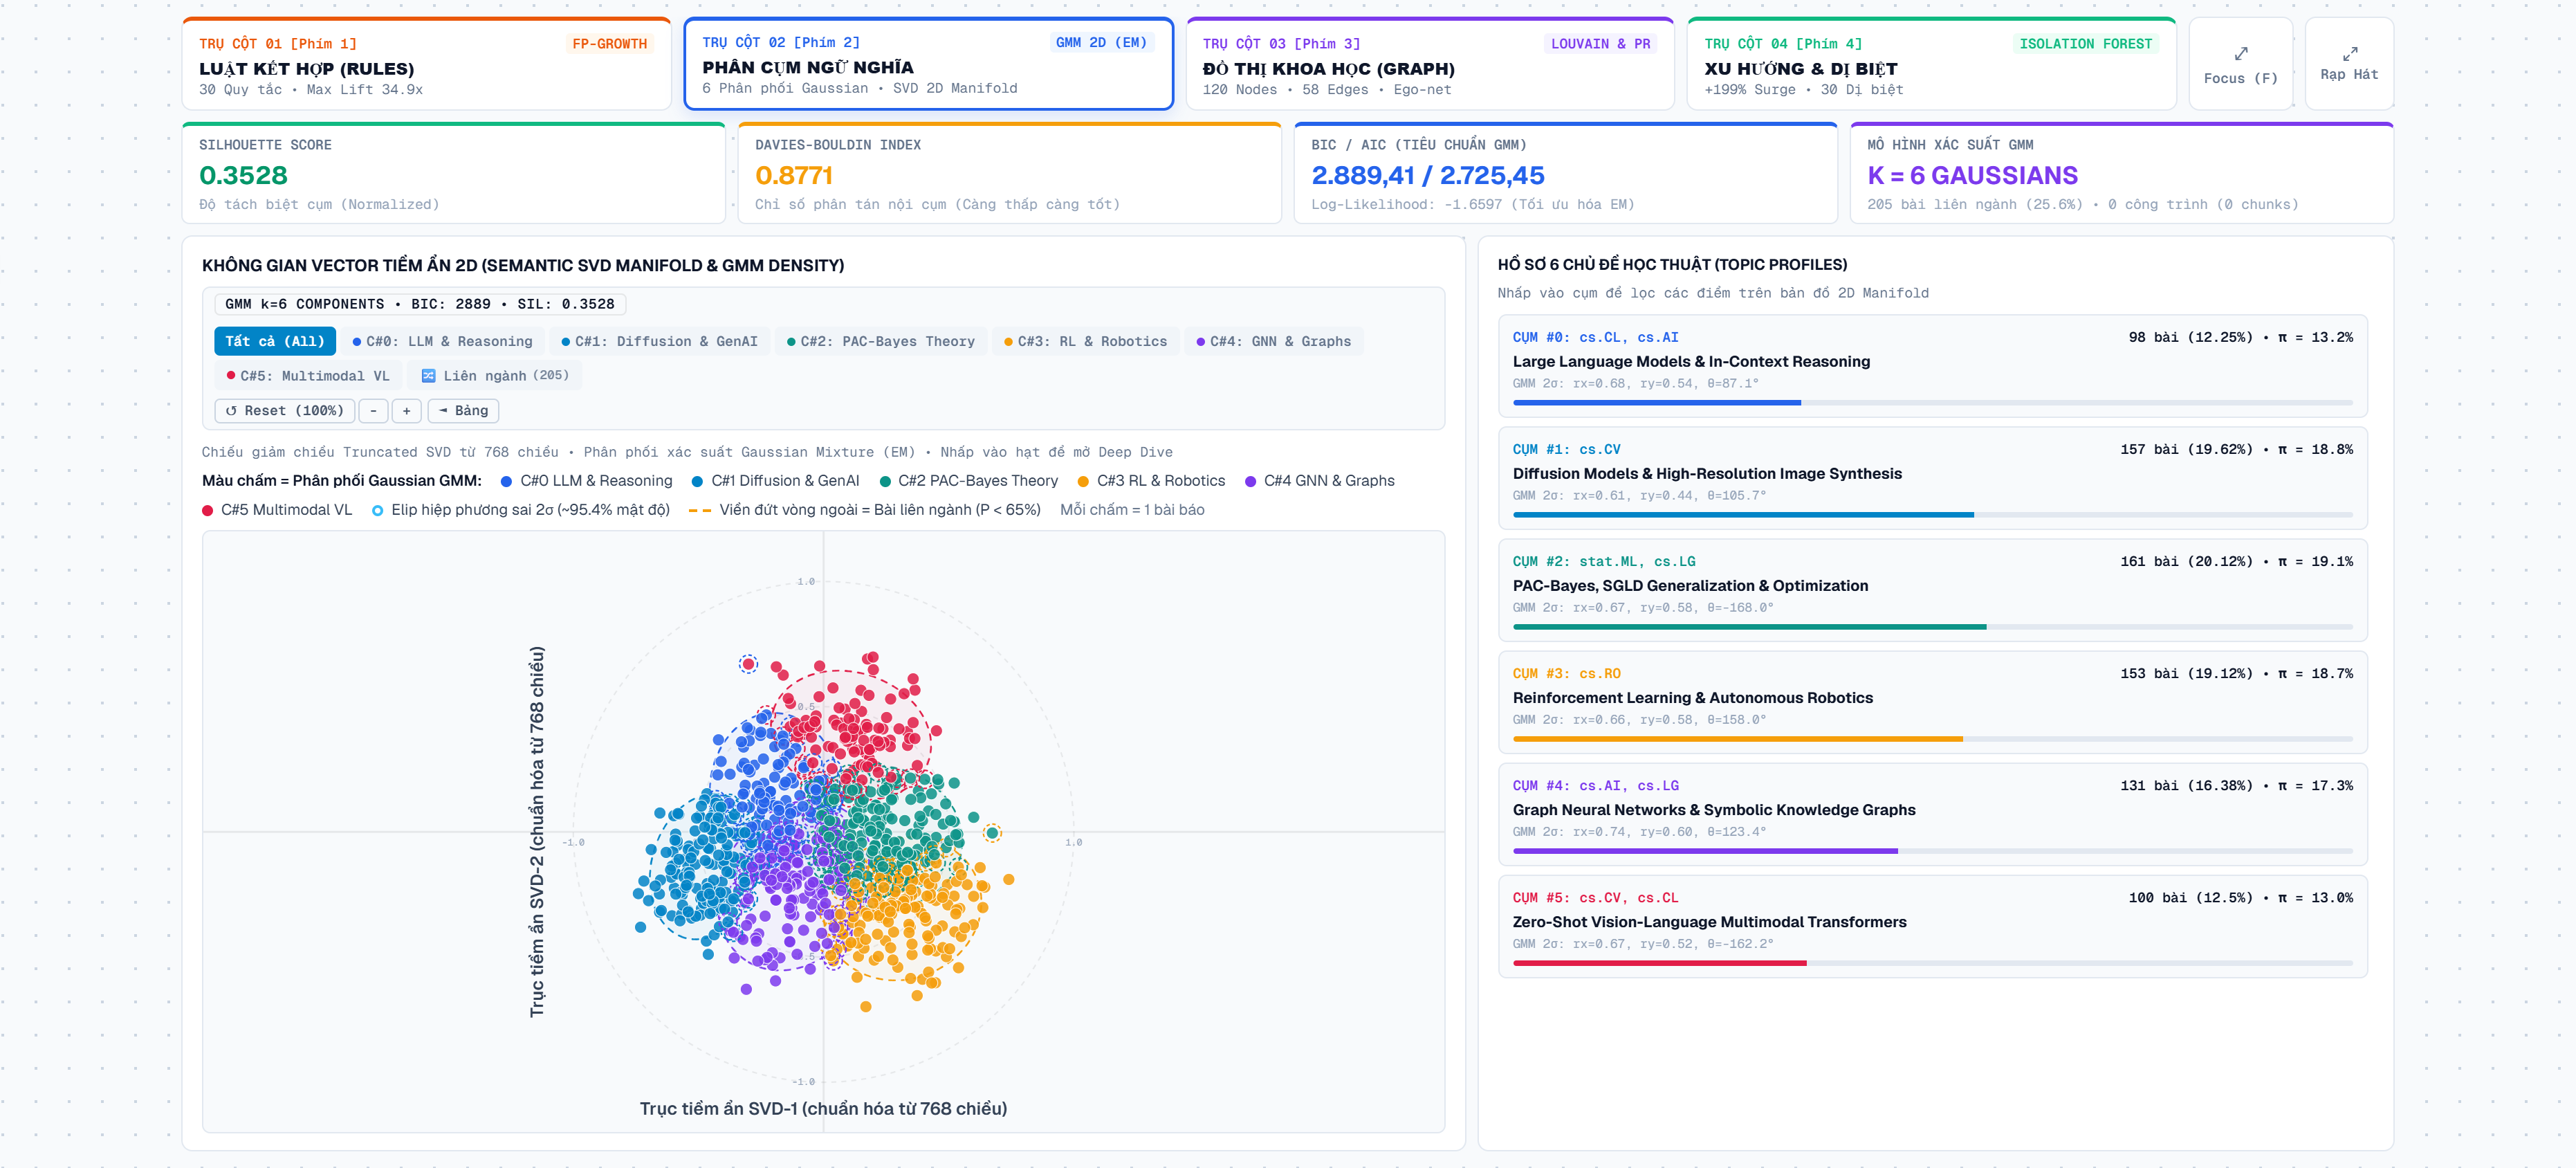
\includegraphics[width=\linewidth,height=0.68\textheight,keepaspectratio]{figures/captured_20261123_082337/06_gmm_clusters.png}
\caption[Giao diện kết quả phân cụm EM GMM trên lát cắt 800 mẫu]{Giao diện kết quả phân cụm EM GMM trên lát cắt 800 mẫu}
\ReportNote{Nguồn: Giao diện phân cụm EM Gaussian Mixture Model ($K=6$) từ \path{evidence/clusters_api.json} và \path{gold/mining/clusters.json} (lát cắt \texttt{SNAP-05}, ngày 20/10/2026, chụp ngày 23/11/2026). Lưu ý nhãn giao diện cũ vẫn hiển thị tên SVD 2D trong phần chú thích của lát cắt này.}
\label{fig:gmm_capture}
\end{figure}
\FloatBarrier

\section{Trụ Cột 3: Khai Phá Mạng Lưới Khoa Học Chế Độ Kép (PageRank và Louvain)}
\label{sec:ch4_graph}

\subsection{Mô Hình Hóa Đồ Thị: Citation DiGraph và Co-authorship Fractional Weight}
\label{sec:ch4_graph_modes}

Trong \path{src/mining/graph_mining.py}, lớp \texttt{ScientificGraphMiner} (giữ bí danh tương thích ngược \texttt{CoauthorshipGraphMiner}) tự động chọn một trong hai chế độ topo đồ thị dựa trên dữ liệu hiện có trên MinIO:
\begin{enumerate}[label=\textbf{\arabic*.}]
  \item \textbf{Chế độ ưu tiên --- Đồ thị Trích dẫn Có hướng (\path{silver/citations.parquet})}: Khi tồn tại các cạnh trích dẫn nội bộ (\texttt{WHERE is\_internal = true}), đồ thị có hướng $G_{\text{cite}} = (V, E)$ được dựng với mỗi nút $v \in V$ là một bài báo và cạnh có hướng $(u \rightarrow v) \in E$ biểu diễn $u$ trích dẫn $v$. Trong chế độ này, trường \texttt{degree} ghi bậc vào (\texttt{in\_degree}) và \texttt{paper\_count} ghi tổng trích dẫn toàn cục (\texttt{citation\_count}).
  \item \textbf{Chế độ dự phòng --- Đồ thị Đồng tác giả Vô hướng Có trọng số Phân đoạn}: Khi không có bảng trích dẫn, mỗi bài báo $p$ có $N_p > 1$ tác giả đóng góp một cạnh vô hướng giữa mọi cặp đồng tác giả $(u, v)$ với trọng số chia đều nghịch đảo số đồng tác giả còn lại nhằm chống lạm phát uy tín từ các bài \textit{hyper-authorship} (tới 144--147 tác giả như đã thấy ở Chương~\ref{chap:data_understanding}):
  \begin{equation}
    W(u, v) = \sum_{p \in P_{uv}} \frac{1}{N_p - 1}, \qquad N_p > 1
    \label{eq:ch4_fractional_weight}
  \end{equation}
  Trong đó: $P_{uv}$ là tập các bài báo mà hai tác giả $u$ và $v$ cùng đứng tên; $N_p$ là tổng số tác giả của bài báo $p$. Hệ số $1/(N_p - 1)$ bảo đảm tổng trọng số một bài báo đóng góp vào mỗi tác giả luôn cân bằng theo mức tham gia.
\end{enumerate}

\subsection{Thuật Toán Damped PageRank và Tối Ưu Modularity Louvain}
\label{sec:ch4_pagerank_louvain}

Để đo uy tín lan truyền trên toàn mạng lưới thay vì chỉ đếm bậc cục bộ, hệ thống áp dụng \textbf{Damped PageRank}~\cite{page1999pagerank} thông qua \texttt{nx.pagerank(G, alpha=0.85)}:
\begin{equation}
  \mathrm{PR}(v) = \frac{1 - \alpha}{|V|} + \alpha \sum_{u \in \mathcal{N}_{\text{in}}(v)} \frac{w(u, v)}{\sum_{z \in \mathcal{N}_{\text{out}}(u)} w(u, z)} \, \mathrm{PR}(u)
  \label{eq:ch4_pagerank}
\end{equation}
Trong đó: $\alpha = 0.85$ là hệ số giảm chấn; $|V|$ là tổng số nút trong đồ thị; $\mathcal{N}_{\text{in}}(v)$ là tập nút trỏ tới $v$; $\mathcal{N}_{\text{out}}(u)$ là tập nút mà $u$ trỏ tới; $w(u, v)$ là trọng số cạnh $(u, v)$ (bằng 1 trên đồ thị trích dẫn nhị phân hoặc $W(u, v)$ trên đồ thị đồng tác giả). Song song đó, cấu trúc cộng đồng học thuật được phát hiện bằng thuật toán \textbf{Louvain}~\cite{blondel2008fast} (\texttt{louvain\_communities(G\_undir, seed=42)}) nhằm cực đại hóa độ đo \textbf{Modularity $Q$}:
\begin{equation}
  Q = \frac{1}{2m} \sum_{i, j} \left[ A_{ij} - \frac{k_i k_j}{2m} \right] \delta(c_i, c_j)
  \label{eq:ch4_louvain}
\end{equation}
Trong đó: $A_{ij}$ là trọng số cạnh giữa hai nút $i$ và $j$; $k_i = \sum_j A_{ij}$ là tổng trọng số bậc của nút $i$; $m = \frac{1}{2}\sum_{i,j} A_{ij}$ là tổng trọng số toàn đồ thị; $\delta(c_i, c_j) = 1$ nếu nút $i$ và $j$ thuộc cùng cộng đồng $c_i = c_j$, ngược lại bằng $0$.

\subsection{Kết Quả Thực Nghiệm Mạng Lưới và Nút Thắt Thời Gian}
\label{sec:ch4_graph_results}

Ở lần chạy toàn hồ ngày 04/11/2026 (\texttt{SNAP-06A}), \texttt{ScientificGraphMiner} tiêu tốn \textbf{116.39 giây --- chiếm 49.6\% tổng thời gian 234.57 giây} của toàn bộ \texttt{MiningEngine}, xác nhận đây là nút thắt cổ chai CPU lớn nhất do phép lặp hội tụ PageRank và phân rã Louvain trên đồ thị hàng chục nghìn nút (\path{logs/run/backend.log}). Bảng~\ref{tab:graph_influencers} đối chiếu các cấu hình đồ thị thực chứng thu được từ dữ liệu Gold.

\begin{table}[!htbp]
\centering
\footnotesize
\setlength{\tabcolsep}{3pt}
\caption[Cấu trúc mạng lưới khoa học chế độ kép và Top nút uy tín PageRank]{Cấu trúc mạng lưới khoa học chế độ kép (Trích dẫn có hướng vs Đồng tác giả) và Top nút uy tín PageRank}
\label{tab:graph_influencers}
\begin{tabularx}{\linewidth}{|>{\raggedright\arraybackslash}p{28mm}|>{\centering\arraybackslash}p{14mm}|>{\centering\arraybackslash}p{15mm}|>{\centering\arraybackslash}p{16mm}|L|>{\raggedright\arraybackslash}p{34mm}|}
\hline
\textbf{Chế độ đồ thị} & \textbf{Nút ($|V|$)} & \textbf{Cạnh ($|E|$)} & \textbf{Cộng đồng} & \textbf{Nút uy tín tiêu biểu} & \textbf{PageRank \& Chỉ số chi tiết} \\ \hline
\textbf{Trích dẫn Có hướng} (hạng 1) & 8,892 & 86,295 & 92 & Vaswani et al. (\textit{Attention Is All You Need}~\cite{vaswani2017attention}) & \textbf{0.012632}; \path{in_degree} = 1,213; \path{cites} = 26,678 \\ \hline
\textbf{Trích dẫn Có hướng} (hạng 2) & 8,892 & 86,295 & 92 & Matthew E. Peters et al. (\textit{ELMo}) & \textbf{0.008603}; \path{in_degree} = 900; \path{cites} = 12,264 \\ \hline
\textbf{Trích dẫn Có hướng} (hạng 3) & 8,892 & 86,295 & 92 & Jakub\r{u}v, Jan et al. (\textit{Exploiting GenAI...}) & \textbf{0.007782}; \path{in_degree} = 1,145; \path{cites} = 78,459 \\ \hline
\textbf{Mạng Đồng tác giả} (snapshot cục bộ) & 35,117 & 130,082 & 3,740 & Yang Liu (hạng 1) / Hao Chen (hạng 2) & 0.000509 (\path{deg}=237, 38 bài) / 0.000463 (\path{deg}=189, 32 bài) \\ \hline
\textbf{Chỉ số mở rộng} (\path{citation_metrics.parquet}) & 29,523 tác giả & 10,000 bài nền & -- & Từ điển PageRank phục vụ thí nghiệm \texttt{EXP-04} & Kết hợp đồ thị bài báo và tác giả (Chương~\ref{chap:evaluation}) \\ \hline
\end{tabularx}
\ReportNote{Nguồn: \path{data/gold/mining/graph_coauthorship.json} (mật độ \path{density = 0.001092}, 29,911 bài lập chỉ mục), snapshot mạng đồng tác giả 35,117 tác giả, và \path{data/gold/graphs/citation_metrics.parquet}. Trong lần chạy sản xuất 04/11/2026 (\texttt{SNAP-06A}), \texttt{ScientificGraphMiner} tiêu tốn 116.39 giây (49.6\% tổng thời gian 234.57 giây).}
\end{table}


Đáng chú ý, hằng số chuẩn hóa PageRank trần trong \texttt{RetrievalService} (\texttt{\_MAX\_PAGERANK = 0.012632}) được kế thừa trực tiếp từ giá trị PageRank đỉnh của công trình nền tảng \textit{Attention Is All You Need}~\cite{vaswani2017attention} (0.012632) trong đồ thị trích dẫn có hướng ở Bảng~\ref{tab:graph_influencers}.

\FloatBarrier
\section{\texorpdfstring{Trụ Cột 4: Động Lượng Thị Phần $\Delta\text{Share}$ và Phát Hiện Bất Thường Isolation Forest}{Tru Cot 4: Dong Luong Thi Phan Delta Share va Phat Hien Bat Thuong Isolation Forest}}
\label{sec:ch4_trends_anomalies}

\subsection{\texorpdfstring{Cửa Sổ Thứ Tự Thời Gian \texttt{dense\_rank()} và Động Lượng Thị Phần}{Cua So Thu Tu Thoi Gian dense\_rank() va Dong Luong Thi Phan}}
\label{sec:ch4_share_momentum}

Nhằm khắc phục triệt để hiện tượng dồn cục theo tháng thu hoạch đã chứng minh ở Chương~\ref{chap:data_understanding} (Mục~\ref{sec:ch3_insight3}), lớp \texttt{TrendAnomalyMiner} (\path{src/mining/trend_anomaly_mining.py}) xếp hạng các tháng thực tế có quan sát giảm dần bằng hàm cửa sổ SQL \texttt{DENSE\_RANK()} (Đoạn mã~\ref{lst:ch4_dense_rank}).

\begin{lstlisting}[language=SQL, caption={Xep hang cac thang quan sat thuc te bang DENSE\_RANK nham loai bo sai lech dot thu thap}, label={lst:ch4_dense_rank}]
-- Order observed publication months sequentially without fixed calendar bias
WITH ym_ranked AS (
    SELECT
        SUBSTR(published_date, 1, 7) AS ym,
        DENSE_RANK() OVER (ORDER BY SUBSTR(published_date, 1, 7) DESC) AS m_rank
    FROM fulltext_view
    WHERE published_date >= '2020-01-01'
    GROUP BY SUBSTR(published_date, 1, 7)
)
\end{lstlisting}

Cửa sổ \texttt{recent} gồm 3 tháng quan sát mới nhất (\texttt{m\_rank <= 3}), cửa sổ \texttt{previous} gồm 3 tháng quan sát kề trước (\texttt{m\_rank BETWEEN 4 AND 6}), và chỉ đánh giá các chuyên ngành có tổng lũy kế \texttt{all\_time\_total >= 40}. Động lượng của chuyên ngành $c$ được chuẩn hóa theo \textbf{thị phần tương đối} (\textit{Share-Normalized Momentum}):
\begin{align}
  s_{\text{rec}}(c) &= \frac{\operatorname{Count}_{\text{rec}}(c)}{\sum_{k} \operatorname{Count}_{\text{rec}}(k)}, &
  s_{\text{prev}}(c) &= \frac{\operatorname{Count}_{\text{prev}}(c)}{\sum_{k} \operatorname{Count}_{\text{prev}}(k)}, \notag \\
  \Delta s(c) &= 100 \times \left(s_{\text{rec}}(c) - s_{\text{prev}}(c)\right)\,[\%], &
  g(c) &= 100 \times \frac{s_{\text{rec}}(c) - s_{\text{prev}}(c)}{s_{\text{prev}}(c)}\,[\%].
  \label{eq:ch4_share_momentum}
\end{align}
Trong đó: $\operatorname{Count}_{\text{rec}}(c)$ và $\operatorname{Count}_{\text{prev}}(c)$ là số bài của chuyên ngành $c$ trong cửa sổ gần nhất và cửa sổ trước đó; $s_{\text{rec}}(c), s_{\text{prev}}(c)$ là thị phần tương ứng trên toàn tập bài trong cửa sổ; $\Delta s(c)$ là biến thiên thị phần tính theo điểm phần trăm; $g(c)$ là tốc độ tăng trưởng thị phần tương đối (nếu $s_{\text{prev}}(c) = 0$ và $s_{\text{rec}}(c) > 0$, gán $g(c) = 100.0\%$). Nhãn trạng thái được gán thành \texttt{SURGING} nếu $g(c) > 15.0\%$ hoặc $\Delta s(c) > 1.5$; \texttt{DECLINING} nếu $g(c) < -15.0\%$ hoặc $\Delta s(c) < -1.5$; và \texttt{STABLE} cho các trường hợp còn lại.

\subsection{\texorpdfstring{Isolation Forest 5 Chiều trên Thang $\ln(1+x)$ và Lý Giải Tự Động}{Isolation Forest 5 Chieu tren Thang ln(1+x) va Ly Giai Tu Dong}}
\label{sec:ch4_iforest}

Từ kết luận kiểm định đuôi dài ở Chương~\ref{chap:data_understanding}, \path{TrendAnomalyMiner} trích xuất vector đặc trưng 5 chiều $\mathbf{x}_i = [\text{math}, \text{words}, \text{sections}, \text{authors}, \text{categories}]^\top$, nén phi tuyến qua $\tilde{\mathbf{x}}_i = \ln(1 + \mathbf{x}_i)$ (\path{np.log1p}) và huấn luyện mô hình \path{IsolationForest(contamination=0.02, random_state=42, n_estimators=100)}~\cite{liu2008isolation}. Điểm bất thường lý thuyết của một quan sát $x$ trên mẫu kích thước $n$ được xác định qua độ sâu đường đi trung bình $\mathbb{E}[h(x)]$ trên 100 cây cô lập ngẫu nhiên:
\begin{equation}
  s(x, n) = 2^{-\frac{\mathbb{E}[h(x)]}{c(n)}},
  \qquad
  c(n) = 2 H(n - 1) - \frac{2(n - 1)}{n}
  \label{eq:ch4_iforest}
\end{equation}
Trong đó: $\mathbb{E}[h(x)]$ là độ sâu đường đi trung bình từ gốc đến lá cô lập $x$; $c(n)$ là độ dài đường đi trung bình của tìm kiếm không thành công trên cây tìm kiếm nhị phân có $n$ điểm; $H(i) \approx \ln(i) + \gamma_{\text{Euler}}$ là số điều hòa thứ $i$. Trong cài đặt Scikit-learn (\texttt{clf.score\_samples}), giá trị xuất ra mang dấu âm (như $-0.7035$, $-0.6906$), với giá trị càng âm tương ứng $\mathbb{E}[h(x)]$ càng ngắn và mức độ dị biệt cấu trúc càng cao. Hệ thống đồng thời tự động sinh danh sách lý giải đa nhãn \texttt{anomaly\_reasons} khi bài báo vượt ngưỡng toán học (\texttt{math > 1,000}: \textit{Math-Heavy Theory}), độ dài (\texttt{words > 25,000}: \textit{Monograph / Mega-Survey}), quy mô nhóm (\texttt{authors > 15}: \textit{Hyper-Authorship Collaboration}), hoặc đa ngành cực đoan (\texttt{categories >= 4}).

\subsection{Kết Quả Thực Nghiệm Xu Hướng và Ngoại Lai}
\label{sec:ch4_trends_results}

Ở lần chạy sản xuất toàn hồ ngày 04/11/2026 (\texttt{SNAP-06A}), \texttt{TrendAnomalyMiner} hoàn tất trong \textbf{2.89 giây} trên \textbf{71,927 bài báo}, cô lập \textbf{1,000 bài báo ngoại lai hàng đầu} (\texttt{contamination = 0.02}) và theo dõi động lượng trên \textbf{48 chuyên ngành} đủ ngưỡng \texttt{all\_time >= 40} (\path{logs/run/backend.log}). Bảng~\ref{tab:anomalies} tổng hợp các biến động động lượng nổi bật và các bài báo ngoại lai tiêu biểu từ \path{data/gold/mining/trends_anomalies.json}.
\begin{table}[!htbp]
\centering
\footnotesize
\setlength{\tabcolsep}{3pt}
\caption[Kết quả động lượng thị phần và bất thường Isolation Forest]{Kết quả động lượng thị phần (\texorpdfstring{$\Delta\text{Share}$}{Delta Share}) và các bài báo bất thường cấu trúc tiêu biểu (\texttt{trends\_anomalies.json})}
\label{tab:anomalies}
\begin{tabularx}{\linewidth}{|>{\raggedright\arraybackslash}p{24mm}|>{\raggedright\arraybackslash}p{22mm}|>{\centering\arraybackslash}p{24mm}|L|>{\raggedright\arraybackslash}p{34mm}|}
\hline
\textbf{Mã / Ngành} & \textbf{Loại kết quả} & \textbf{Giá trị định lượng} & \textbf{Đặc trưng nổi bật} & \textbf{Trạng thái / Nhãn lý giải} \\ \hline
\path{cs.CV} & Động lượng & \texttt{growth = +123.43\%} & \path{recent = 722}, \path{prev = 6}, \path{all = 3,021} & \texttt{SURGING} \\ \hline
\path{cs.AI} & Động lượng & \texttt{growth = +198.94\%} & \path{recent = 161}, \path{prev = 1}, \path{all = 625} & \texttt{SURGING} \\ \hline
\path{cs.CL} & Động lượng & \texttt{growth = +69.89\%} & \path{recent = 366}, \path{prev = 4}, \path{all = 1,858} & \texttt{SURGING} \\ \hline
\path{cs.LG} & Động lượng & \texttt{growth = +38.64\%} & \path{recent = 672}, \path{prev = 9}, \path{all = 3,093} & \texttt{SURGING} \\ \hline
\path{cs.RO} & Động lượng & \texttt{growth = -81.43\%} & \path{recent = 160}, \path{prev = 16}, \path{all = 879} & \texttt{DECLINING} \\ \hline
\path{cs.IR} & Động lượng & \texttt{growth = -3.45\%} & \path{recent = 52}, \path{prev = 1}, \path{all = 310} & \texttt{STABLE} \\ \hline
\path{arXiv:2206.08756} & Ngoại lai IF (\#1) & \path{score = -0.7035} & 1,600 công thức, 15,279 từ, 6 nhãn ngành & Math-Heavy + Extreme Multidisciplinary \\ \hline
\path{arXiv:2501.05498} & Ngoại lai IF (\#2) & \path{score = -0.6906} & 5,470 công thức, 74,303 từ & Extreme Math + Mega-Survey Monograph \\ \hline
\path{arXiv:2401.13216} & Ngoại lai IF (\#3) & \path{score = -0.6865} & 3,732 công thức, 26,576 từ, 4 nhãn ngành & Math-Heavy + Mega-Survey + 4 Categories \\ \hline
\path{arXiv:2411.15221} & Ngoại lai đa tác giả & \path{score = -0.6826} & 144 đồng tác giả, 24,057 từ, 20 công thức & Hyper-Authorship Collaboration \\ \hline
\end{tabularx}
\ReportNote{Nguồn: \path{data/gold/mining/trends_anomalies.json} (lát cắt cục bộ 29,911 bài, 260 ngoại lai, 26 chuyên ngành). Trên lần chạy sản xuất 04/11/2026 (\texttt{SNAP-06A}), \texttt{TrendAnomalyMiner} xử lý toàn bộ 71,927 bài trong 2.89 giây, phát hiện 1,000 ngoại lai hàng đầu (\path{contamination = 0.02}) và theo dõi 48 chuyên ngành đạt ngưỡng \path{all_time >= 40}.}
\end{table}

